\section{Resultados e Discussão}\label{sec:resultados}

\subsection{Comparação entre as tecnologias}\label{sec:comparacao}

\begin{table}[t]
  \caption{Métricas por motor com as taxas nominais}
  \label{tab:metricas}
  \centering
  \setlength{\tabcolsep}{4pt}
  \begin{tabular}{@{}lrrcc@{}}
    \toprule
    Motor & $\lambda$ (\pcmh) & MTBF (h) & $F(1\,\mathrm{h})$ & $R(1000\,\mathrm{h})$ \\
    \midrule
    Pistão & 12,4 & 8026 & \num{1.24e-4} & 0,883 \\
    Turboélice & 0,15 & 666667 & \num{1.5e-6} & 0,9985 \\
    Turbofan & 0,20 & 499903 & \num{2.0e-6} & 0,9980 \\
    \bottomrule
  \end{tabular}
\end{table}

\begin{figure}[t]
  \centering
  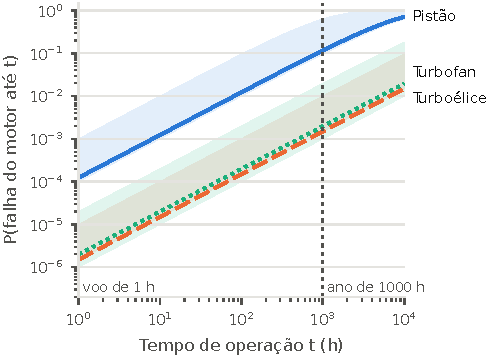
\includegraphics[width=\columnwidth]{figures/fig_prob_falha_tempo}
  \caption{Probabilidade de falha do motor até $t$. Linha: taxa nominal; faixa: da taxa mínima à máxima da Tabela~\ref{tab:taxas}.}
  \label{fig:tempo}
\end{figure}

Com as taxas nominais, o motor a pistão tem 83 vezes a probabilidade de falha do turboélice em um voo de 1~h e 62 vezes a do turbofan (Tabela~\ref{tab:metricas}).
Em um ano de 1000~h, a chance de ao menos uma falha é de 12\% no pistão e de 0,15\% a 0,20\% nos motores a turbina.
Mesmo no mínimo de sua faixa (10 \pcmh), o pistão falha 5 vezes mais que o turbofan e 10 vezes mais que o turboélice tomados no máximo das faixas deles (Fig.~\ref{fig:tempo}).
Entre os dois motores a turbina, o modelo não estabelece uma ordem: o turbofan tem taxa nominal um pouco maior, mas as faixas, de 0,15 a 1 e de 0,10 a 2 \pcmh, se sobrepõem quase por inteiro.

A redundância interna pouco altera o comportamento no tempo.
No pistão, a taxa equivalente fica em 12,40 \pcmh{} tanto em 1~h quanto em 1000~h, e o MTBF sem reparo (8026~h) fica perto do MTBF com o par restaurado a cada voo (8065~h).
Na análise de sensibilidade, a taxa total domina: quando $\lambda$ percorre a faixa, $F(1\,\mathrm{h})$ varia 10 vezes no pistão, 6,7 vezes no turboélice e 20 vezes no turbofan.
Já $\beta$ e $\lambda_u$ não mudam $F(1\,\mathrm{h})$, efeito da preservação da taxa publicada, e só alteram o Pareto.

\subsection{Subsistemas críticos}\label{sec:pareto}

\begin{figure*}[t]
  \centering
  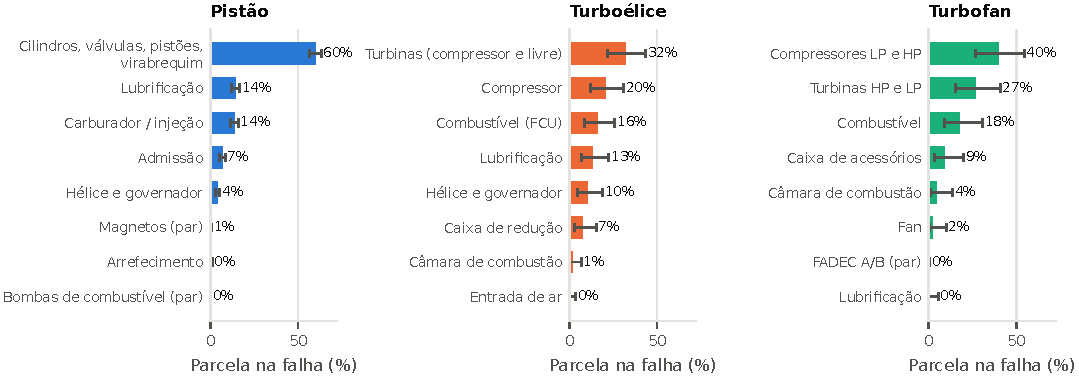
\includegraphics[width=\textwidth]{figures/fig_pareto_blocos}
  \caption{Parcela de cada subsistema na falha do motor em um voo de 1~h, com o intervalo de Jeffreys de 95\%.}
  \label{fig:pareto}
\end{figure*}

No pistão, o núcleo mecânico (cilindros, válvulas, pistões e virabrequim) responde por 60\% das falhas (IC 95\% de 57\% a 63\%), seguido de lubrificação e carburador/injeção, com 14\% cada (Fig.~\ref{fig:pareto}).
Com admissão e hélice, os cinco blocos em série sem redundância chegam a 99\%, como a proposta esperava.
Os pares redundantes ficam no fim do Pareto, com 0,6\% para os magnetos e 0,07\% para as bombas.
Nas turbinas, com 69 e 45 registros, os intervalos são largos. No turboélice, as turbinas lideram com 32\% (22\% a 43\%), seguidas do compressor, com 20\%, e do combustível (FCU), com 16\%.
No turbofan, lideram os compressores, com 40\% (27\% a 55\%), as turbinas, com 27\%, e o combustível, com 18\%; o fan, com um único registro, fica com 2\%.
Nos dois motores a turbina, as partes rotativas do gerador de gás concentram mais da metade das falhas.


\subsection{Redundância}\label{sec:redundancia}

\begin{table}[t]
  \caption{Efeito dos pares redundantes ($\beta=0{,}1$)}
  \label{tab:redundancia}
  \centering
  \setlength{\tabcolsep}{2.5pt}
  \begin{tabular}{@{}lrrcr@{}}
    \toprule
    Par & $n_p$ & $\lambda_u$ (\pcmh) & Ganho & Sem o par \\
    \midrule
    Magnetos (pistão) & 102 & 0,72 & 10$\times$ & +5,2\% \\
    Bombas (pistão) & 12 & 0,085 & 10$\times$ & +0,6\% \\
    FADEC A/B (turbofan) & 1 & 0,0022 & 10$\times$ & +1,0\% \\
    \bottomrule
    \multicolumn{5}{@{}l}{\footnotesize Ganho: $F$ de uma unidade sobre $F$ do par.} \\
    \multicolumn{5}{@{}l}{\footnotesize Sem o par: aumento em $F(1\,\mathrm{h})$ do motor.}
  \end{tabular}
\end{table}

Os pares reduzem em cerca de 10 vezes a probabilidade de perder a função (Tabela~\ref{tab:redundancia}).
O ganho é limitado por $\beta$: com $\beta=0{,}1$, quase toda a probabilidade de falha do par vem da causa comum, e o ganho fica perto de $1/\beta$.
Sem os dois pares, o motor a pistão teria uma probabilidade de falha em 1~h 5,8\% maior, $\num{1.31e-4}$ contra $\num{1.24e-4}$.
A coluna ``sem o par'' é também o risco de voar com uma unidade já inoperante: decolar com um magneto em pane eleva $F(1\,\mathrm{h})$ em 5,2\%, e com uma bomba em pane, em 0,6\%.
No turbofan, o FADEC tem um único registro, e a taxa da unidade vai de 0,0002 a 0,011 \pcmh{} no intervalo de Jeffreys; mesmo no máximo, a duplicação quase não altera o resultado.
Como falhas que o próprio par tolera raramente terminam em acidente, as taxas dos pares tendem a estar subestimadas.

\begin{figure}[t]
  \centering
  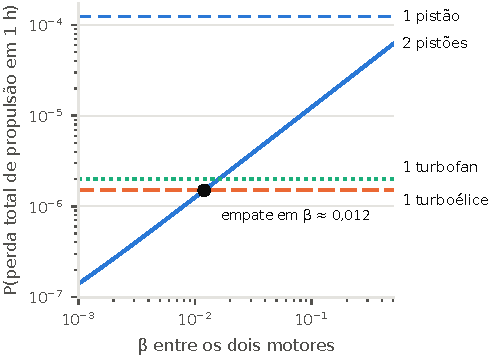
\includegraphics[width=\columnwidth]{figures/fig_bimotor}
  \caption{Probabilidade de perda total de propulsão em 1~h em função de $\beta$ entre os dois motores, com taxas nominais.}
  \label{fig:bimotor}
\end{figure}

Com dois motores, a perda total de propulsão exige que os dois falhem no mesmo voo.
Se as falhas fossem independentes, dois pistões perderiam toda a propulsão com probabilidade de $\num{1.5e-8}$ por hora, muito abaixo de um motor a turbina.
A causa comum entre os motores muda esse quadro (Fig.~\ref{fig:bimotor}).
Com as taxas nominais, o bimotor a pistão só é mais seguro que um turboélice se $\beta<0{,}012$, e mais seguro que um turbofan se $\beta<0{,}016$.
Com a taxa da turbina nos extremos da faixa, o limite vai de 0,012 a 0,081 contra o turboélice e de 0,008 a 0,161 contra o turbofan, na parte de baixo da faixa usual de $\beta$, de 0,01 a 0,3.
O bimotor também dobra a chance de ter alguma falha de motor no voo ($\num{2.5e-4}$ por hora), e o modelo conta só a perda total de propulsão, não a dificuldade de controlar o avião com um motor parado.

\subsection{Consequência da falha no NTSB}\label{sec:empirico}

\begin{figure}[t]
  \centering
  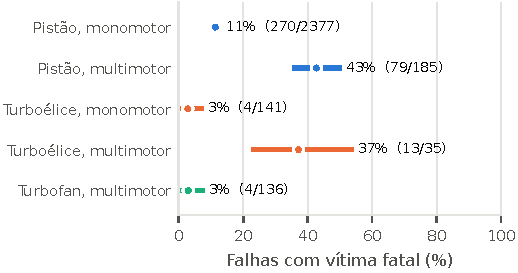
\includegraphics[width=\columnwidth]{figures/fig_ntsb_prob_fatal}
  \caption{Falhas de motor com vítima fatal no NTSB (2008--2026), por tecnologia e número de motores, com intervalo de Wilson de 95\%.}
  \label{fig:fatal}
\end{figure}

A Fig.~\ref{fig:fatal} dá uma medida empírica dessa dificuldade.
Nos multimotores a pistão, 43\% das falhas de motor registradas tiveram vítima fatal, contra 11\% nos monomotores; no turboélice, 37\% (13 de 35) contra 2,8\% (4 de 141).
A comparação é condicionada ao registro: no multimotor, a falha que termina em pouso normal raramente entra na base, enquanto no monomotor quase toda falha termina em pouso forçado.
Ainda assim, a falha de um motor de multimotor que chega ao NTSB é das mais graves, o que é coerente com a perda de controle por tração assimétrica, que o RBD não modela.
O monomotor turboélice tem a menor proporção (2,8\%), próxima à do turbofan (2,9\%).
Junto com o limite de $\beta$, isso indica que dois motores a pistão não equivalem, na prática, a um motor a turbina.
As falhas por combustível ficaram fora: são 1532 no pistão, 174 delas com vítima fatal.

\subsection{Taxa constante}\label{sec:weibull}

No pistão, com 903 casos e 4000 controles, a forma estimada pelo TSO é 0,99 (IC 95\% de 0,94 a 1,05; $p=0{,}79$ para $k=1$), compatível com a taxa constante do RBD entre revisões.
Pelo TSN, a forma é 1,08 (1,02 a 1,13), um desgaste leve ao longo da vida do motor: nos três quartis mais altos de TSN, a chance de falha é de 1,4 a 1,5 vez a do primeiro.
No turboélice, com 32 falhas com TSO, a forma é 1,28 (0,97 a 1,59), e no turbofan quase nenhum monomotor tem horas registradas.
O teste supõe que os controles tenham a idade de motor da frota.

\subsection{Limitações}\label{sec:limitacoes}

A estimativa por \eqref{eq:fracao} supõe que a chance de uma falha entrar no NTSB é a mesma para todos os blocos.
O NTSB registra sobretudo acidentes (no pistão, 2529 das 2562 falhas), e as frações descrevem as falhas que levaram a acidente ou incidente investigado, e não todas as falhas em voo.
Os 535 achados genéricos excluídos são supostos distribuídos entre os blocos na mesma proporção dos classificados.
Os motores entram por tipo, e não por modelo, e nas turbinas os blocos sem registro ficam com fração nula.
A taxa do turbofan vem do fabricante, e a do pistão mistura fabricantes e modelos da frota australiana, e não só o O-540.
